\chapter{Test}
I dette afsnit følger selve testen.
\section{Testcases}
Dette afsnit er delt op i  2 dele. Hardware og software:\\
%%%%%%%%%%%%%%%%%%%%%%%%%%%%%%%%%%
%%% HARDWARE                   %%%
%%%%%%%%%%%%%%%%%%%%%%%%%%%%%%%%%%
\subsection{Hardware}
I dette afsnit forklares hvordan enhedstest af hardware udføres.
\subsubsection{SM}
\begin{table}[H]
\centering
\begin{tabular}{| p{1cm}  | p{4.5cm} | p{8cm} |}
\hline
Case &Formål &Udførelse\\\hline
1 &Indstil Accelerometer &Der skrives 0x06 på P15[2:0]\\\hline
2 &Verificer RS232 &Der sættes en jumper mellem RX\_out og TX\_out og derefter sendes der 5 forskellige chars via UART\\\hline
\end{tabular}
\end{table}
\subsubsection{VBTE}
\begin{table}[H]
\centering
\begin{tabular}{| p{1cm}  | p{4.5cm} | p{8cm} |}
\hline
Case &Formål &Udførelse\\\hline
1 &At teste ventilkreds &Der toggles 5V med 500ms interval ud fra PSoC'en på ben P0\_0 og P0\_2. Der lyttes på ventilerne for at bekræfte at de åbner og lukker.\\\hline
2 &At teste transmitterkreds &Der sendes et 40kHz signal fra funktionsgeneratoren med 12Vp-p. Der læses med oscilloskop på receiveren og det valideres om signalet bliver transmitteret.\\\hline
3 &At teste receiverkredsen & Der sendes burst fra transmitterkredsen med 500ms interval med en varighed på $\sim$250$\mu$s. Der indsættes to analoge pinde i PSoCdesignet der kobles til udgangen på PGA'en og udgangen af mixeren. Signalet valideres med oscilloskopbilleder.\\\hline
\end{tabular}
\end{table}
%%%%%%%%%%%%%%%%%%%%%%%%%%%%%%%%%%
%%% SOFTWARE                   %%%
%%%%%%%%%%%%%%%%%%%%%%%%%%%%%%%%%%
\subsection{Software}
I dette afsnit forklares hvordan enhedstests af hardware udføres.
\subsubsection{SM}
\begin{table}[H]
\centering
\begin{tabular}{| p{1cm}  | p{4.5cm} | p{8cm} |}
\hline
Case &Formål &Udførelse\\\hline
1 &getLevel &getLevel kaldes som funktionskald med en stub. Stubben verificere returnværdien.\\\hline
2 &getFromKI &Et program køres hvor getFromKI kaldes i en while løkke. SM modulet sættes sammen med en teststub der sender forskellige kommandoer, 6000 gange. For kommandoer se \textit{Arkitektur}\\\hline
3 &writeToVbte &SM modulet sættes sammen med en I2C teststub der tilføjer 10 til værdien og returner. På SM modulet checkes via Debug menuen hvad der er modtaget.\\\hline
4 &init &init kaldes og der verificeres at en diode på SM modulet aktiveres.\\\hline
5 &autoReg &Der kobles to teststubbe på SM modulet. Derefter vinkles SM modulet således at man opnår $\pm$5 grader. Stubbene returnere skiftevis værdier fra 0 til 100 i trin af 20. Der verificeres at autoReg sender beskeder ud via et display monteret på teststubbe.\\\hline
6 &convertToEnum &Der indsættes værdier fra 2000 til 4000 i trin af 17. Der opserveres på returværdier. \\\hline
7 &convertToValue &Der indsættes alle værdier i Hældningsenum beskrevet i \textit{Arkitektur}. Der opserveres på returværdier.\\\hline
\end{tabular}
\end{table}
\subsubsection{VBTE}
\begin{table}[H]
\centering
\begin{tabular}{| p{1cm}  | p{4.5cm} | p{8cm} |}
\hline
Case &Metode &Udførelse\\\hline
1 &SendBurst &Metoden kaldes i intervaller på 500ms og der måles med osciloskop på ben P0\_1 at der bliver sendt burst's med en varighed på $\sim$250$\mu$s og med en frekvens på $\sim$40kHz.\\\hline
2  &CalculateDistance & Metoden kaldes 100 gange med forskellige inputværdier. Outputtet ligges i et array og der valideres på disse værdier.\\\hline
3 &ConvertMMtoPercent & Metoden kaldes 100 gange med forskellige inputværdier. Outputtet ligges i et array og der valideres på disse værdier.\\\hline
4 & ChangeState & Metoden kaldes med alle forskellige slags input og 3 værdier uden for input. Der lyttes på ventilerne og der valideres om de åbner/lukker som de skal.\\\hline
5 & I2C\_handle & Der anvendes en stub der agerer som SM. Denne sender alle værdier fra protokollen samt 3 værdier uden for protokollen. Der kontrolleres om der modtages alle værdier korrekt ved at udskrive dem på displayet. Der kontrolleres også om den rigtige værdi sendes retur til SM stub'en.\\\hline
6 & I2C\_decode & Metoden kaldes med de forskellige værdier for protokollen samt 3 uden for protokollen. Returværdien kontrolleres for at validere det korrekte state.\\\hline
7 & Init & Metoden kaldes og der kontrolleres om der returneres 1 tilbage.\\\hline
\end{tabular}
\end{table}
%%%%%%%%%%%%%%%%%%%%%%%%
%%%%     KI      %%%%%%%
%%%%%%%%%%%%%%%%%%%%%%%%
\subsubsection{KI}
\begin{table}[H]
\caption{"AKTIVER MANUEL HÆLDNINGSREGULERING\"-knappen}
\centering
\begin{tabular}{| p{1cm}  | p{4.5cm} | p{8cm} |}
\hline
Case &Formål &Udførelse\\\hline
1a &At teste hvorvidt en ændret manuel vinkling sendes ud serielt. &Der indsættes en manuel vinklingsregulering på den grafiske brugergrænseflade. Alle kombinationer af side og værdi afprøves. Der verificeres i terminalen at RS232-klassen udsender værdierne til SM.\\\hline

1b &Det testes hvordan programmet reagerer hvis man efter at have trykket på "AKTIVER MANUEL HÆLDNINGSREGULERING" fortryder sit valg ved tryk på "Cancel"-knappen.&Tryk på knappen. Tryk på "Cancel".\\\hline

1c &Det testes hvordan programmet reagerer hvis der ingen forbindelse er til SM når man forsøger at sætte en manuel hældning. &Tryk på "AKTIVER MANUEL HÆLDNINGSREGULERING" uden forbindelse til SM. Bekræft værdier. Aflæs GUI'en og terminalen.\\\hline
\end{tabular}
\end{table}

\begin{table}[H]
\caption{Opdatering af grafisk brugergrænseflade}
\centering
\begin{tabular}{| p{1cm}  | p{4.5cm} | p{8cm} |}
\hline
Case &Formål &Udførelse\\\hline

2 &At teste hvorvidt en status struct kan requestes fra SM-klassen og sendes til databasen. SM-klassen returnerer en status-stub. Det verificeres i terminalen at dataserver-klassen udsender værdierne til databasen.&Start programmet. Vent til GUI'en opdateres. Aflæs terminalen.\\\hline
\end{tabular}
\end{table}

\begin{table}[H]
\caption{"AKTIVER AUTOMATISK HÆLDNINGSREGULERING\"-knappen}
\centering
\begin{tabular}{| p{1cm}  | p{4.5cm} | p{8cm} |}
\hline
Case &Formål &Udførelse\\\hline
3a &Det testes hvordan programmet reagerer hvis man forsøger at aktivere automatisk regulering, når denne allerede er aktiveret. &Automatisk hældningsregulering skal ikke være aktiveret. Tryk på "AKTIVER AUTOMATISK HÆLDNINGSREGULERING". Aflæs terminalen og GUI'en.\\\hline

3b &Det testes hvordan programmet reagerer hvis man forsøger at aktivere automatisk regulering, når denne ikke er aktiveret. &Der trykkes på knappen "AKTIVER AUTOMATISK HÆLDNINGSREGULERING". Tryk på "YES". Aflæs terminalen og GUI'en.\\\hline

3c &Det testes hvordan programmet reagerer ved tryk på "AKTIVER AUTOMATISK HÆLDNINGSREGULERING" når der ingen forbindelse er til SM.&Tryk på knappen "AKTIVER AUTOMATISK HÆLDNINGSREGULERING". Tryk på "YES". Aflæs GUI.\\\hline
\end{tabular}
\end{table}

\begin{table}[H]
\caption{"LUK BROS\"-knappen}
\centering
\begin{tabular}{| p{1cm}  | p{4.5cm} | p{8cm} |}
\hline
Case &Formål &Udførelse\\\hline
4a &Det testes hvordan programmet reagerer hvis man ønsker at lukke programmet med et tryk på "LUK BROS"-knappen og efterfølgende bekræfter ved tryk på "YES"-knappen.&Tryk på "LUK BROS"-knappen. Tryk på "YES". Aflæs terminalen og GUI'en.\\\hline

4b &Det testes hvordan programmet reagerer hvis man efter tryk på "LUK BROS"-knappen fortryder sit valg ved at trykke "NO".&Tryk på "LUK BROS"-knappen. Tryk på "NO". Aflæs terminalen og GUI'en.\\\hline
\end{tabular}
\end{table}
% Testresultater
\section{Testresultater}
Dette afsnit er delt op i  2 dele baseret på ovenstående tests.\\
%%%%%%%%%%%%%%%%%%%%%%%%%%%%%%%%%%
%%% HARDWARE RESULTATER        %%%
%%%%%%%%%%%%%%%%%%%%%%%%%%%%%%%%%%
\subsection{Hardware}
I dette afsnit findes forventede resultater samt resultater på testcases fra ovenstående hardware kapitel.\\
\subsubsection{SM}
\begin{table}[H]
\centering
\begin{tabular}{| p{1cm}  | p{4cm} | p{6cm} | p{1cm} |}
\hline
Case &Forventet resultat &Resultat &Status\\\hline
1 &Accelerometeret er indstillet. &Det observeres at accelerometeret er indstillet og aktivt. &\begin{Huge}$\surd$\end{Huge}\\\hline
2 &De afsendte chars bliver modtaget via UART. &De afsendte chars blev modtaget via UART. &\begin{Huge}$\surd$\end{Huge}\\\hline
\end{tabular}
\end{table}
\subsubsection{VBTE}
\begin{table}[H]
\centering
\begin{tabular}{| p{1cm}  | p{4cm} | p{6cm} | p{1cm} |}
\hline
Case &Forventet resultat &Resultat &Status\\\hline
1 &Ventilerne åbner og lukker &Det høres tydeligt at ventilerne åbnes og lukkes. &\begin{Huge}$\surd$\end{Huge} \\\hline 
2 &Der ses signal på osciloskopet &Signalet ses på osciloskop. Se \textit{figur \ref{fig:transmittertest}} &\begin{Huge}$\surd$\end{Huge} \\\hline 
3 & Der ses burst efter PGA'en samt "tapper" efter mixeren via. oscilloskop. & Ved første test blev et markant svagere end antaget modtaget. Gain i PGA blev justeret til 32 og testen kunne godkendes. Testresultet ses på \textit{figur \ref{fig:PGA}, \ref{fig:mixer} og \ref{fig:mixer2}} i bilag. &\begin{Huge}$\surd$\end{Huge} \\\hline 
\end{tabular}
\end{table}

%%%%%%%%%%%%%%%%%%%%%%%%%%%%%%%%%%
%%% SOFTWARE RESULTATER        %%%
%%%%%%%%%%%%%%%%%%%%%%%%%%%%%%%%%%
\subsection{Software}
I dette afsnit findes forventede resultater samt resultater på testcases fra ovenstående software kapitel.\\
\subsubsection{SM}
\begin{table}[H]
\centering
\begin{tabular}{| p{1cm}  | p{4cm} | p{6cm} | p{1cm} |}
\hline
Case &Forventet resultat &Resultat &Status\\\hline
1 &Level bliver returneret og verificeret &Level blev returneret og verificeret &\begin{Huge}$\surd$\end{Huge} \\\hline 
2 &teststubben printer til skærmen at alle cases er succesfulde &teststubben printede Success: 6000 &\begin{Huge}$\surd$\end{Huge} \\\hline
3 &Der modtages 13 til 19. &13 til 19 blev modtaget. &\begin{Huge}$\surd$\end{Huge} \\\hline
4 &En LED tænder på SM modulet. &En LED blev tændt. &\begin{Huge}$\surd$\end{Huge} \\\hline
5 &Det observeres at der sendes åben og luk af de forskellige ventiler baseret på de værdier der modtages fra stubbene. &Der blev sendt åben og luk af de forskellige ventiler men i et ud af 20 tilfælde blev der modtaget en værdi større end 100, hvilket medførte en fejlmelding. Dette skyldes noget i hardwaren der behandler I2C. &\begin{Huge}$\surd$\end{Huge} \\\hline
6 &Der modtages værdien svarende til 0 graders hældning for lave værdier hvorefter hele level enum bliver kørt igennem og den efterfølgende returnere 0. &Der blev modtaget 255 indtil hele enum blev kørt igennem hvorefter der blev modtaget 255 igen. &\begin{Huge}$\surd$\end{Huge} \\\hline
7 &Der returneres hældningsværdier svarende til enum vinklingsnavne &Der blev returneret værdier svarende til enums vinklingsnavne. Dog drifter værdien en smule&\begin{Huge}$\surd$\end{Huge} \\\hline
\end{tabular}
\end{table}
\subsubsection{VBTE}
\begin{table}[H]
\centering
\begin{tabular}{| p{1cm}  | p{4cm} | p{6cm} | p{1cm} |}
\hline
Case &Forventet resultat &Resultat &Status\\\hline
1 &Metoden laver et burst på $\sim$250$\mu$s og med en frekvens på $\sim$40kHz & Der er blevet målt med osciloskop på P0\_1. Se resultat på \textit{figur \ref{fig:burstpsoc} og \ref{fig:flereburstpsoc}} i bilag. &\begin{Huge}$\surd$\end{Huge} \\\hline 
2 &Metoden returnerer 100 værdier der stemmer overens med funktionaliteten & Metoden returnerede de forventede værdier. &\begin{Huge}$\surd$\end{Huge} \\\hline 
3 &Metoden returnerer 100 værdier der stemmer overens med funktionaliteten & Metoden returnerede de forventede værdier. &\begin{Huge}$\surd$\end{Huge} \\\hline 
4 &Metoden togler ventilerne som forventet & Ventilerne blev toglet som forventet. &\begin{Huge}$\surd$\end{Huge} \\\hline 
5 &Metoden udskriver værdierne på displayet og svarer SM stub'en & Der blev aflæst det forventede på displayet og svaret til SM stemte overens med forventningerne. &\begin{Huge}$\surd$\end{Huge} \\\hline 
6 &Metoden returnerer de forventede resultater og returnerer luk ventiler ved værdier uden for protokollen& Metoden returnerede de forventede værdier. &\begin{Huge}$\surd$\end{Huge} \\\hline
7 &Metoden returnerer 1 & Metoden returnerede 1. &\begin{Huge}$\surd$\end{Huge} \\\hline  
\end{tabular}
\end{table}
%%%%%%%%%%%%%%%%%%%%%%%%
%%%%     KI      %%%%%%%
%%%%%%%%%%%%%%%%%%%%%%%%
\subsubsection{KI}
\begin{table}[H]
\caption{"AKTIVER MANUEL HÆLDNINGSREGULERING"-knappen}
\centering
\begin{tabular}{| p{1cm}  | p{6cm} | p{5cm} | p{1cm} |}
\hline
Case &Forventet resultat &Resultat &Status\\\hline

1a &I terminalen aflæses det at valget er bekræftiget og at RS232-klassen udsender værdien for kommandoen og dernæst hældningen i overensstemmelse med protokollen\fxnote{indsæt reference til billedet}. I programmet kan det aflæses hvilken værdi der manuelt er indstillet til &Resultatet kan ses i \ref{fig:manuResult} og stemmer overens med forventningerne. &\begin{Huge}$\surd$\end{Huge} \\\hline 

1b &Programmet vender tilbage til stadiet før det første tryk på "AKTIVER MANUEL HÆLDNINGSREGULERING" og trykket har ingen konsekvenser. &Programmet foretog sig intet i relation til trykket. GUI'en er uændret. &\begin{Huge}$\surd$\end{Huge} \\\hline 

1c &Det samme som 1b.&&\begin{Huge}$\surd$\end{Huge}\\\hline
\end{tabular}
\end{table}

\begin{table}[H]
\caption{Opdatering af grafisk brugergrænseflade}
\centering
\begin{tabular}{| p{1cm}  | p{6cm} | p{5cm} | p{1cm} |}
\hline
Case &Forventet resultat &Resultat &Status\\\hline
2 &I terminalen udskrives status-struct-stubben i SM-klassen. Den udskrives efterfølgende igen af dataserver-klassen som den sendes til databasen. Her sendes navnet på skibet og tiden siden sidste opdatering fra SM. Disse er tilføjet Kontrolinterface-klassen.&&\\\hline
\end{tabular}
\end{table}

\begin{table}[H]
\caption{"AKTIVER AUTOMATISK HÆLDNINGSREGULERING"-knappen}
\centering
\begin{tabular}{| p{1cm}  | p{6cm} | p{5cm} | p{1cm} |}
\hline
Case &Forventet resultat &Resultat &Status\\\hline
3a &Det forventes at programmet bringer en dialog op hvori der informeres om at denne reguleringstype allerede er aktiveret. &Programmet reagerede blot med dialogen. \fxnote{indsæt reference til dialog AUTO==ON}. &\begin{Huge}$\surd$\end{Huge} \\\hline

3b &Det forventes at der popper en dialog frem hvor der skal bekræftiges at man ønsker at gå væk fra manuel hældning. Ved bekræftelser udskrives det af RS232-klassen\fxnote{indsæt billede} at kommandoen er sendt. Ved tryk på "NO" lukker dialogen og trykket har ingen videre konsekvens. &Dialogen kom frem og kan ses på figur \fxnote{indsæt MANUELBEKRÆFT-dialog}&\begin{Huge}$\surd$\end{Huge}\\\hline

3c &Det forventes at der poppe en dialog op som i 3b, men at der ved tryk på "YES" intet sker i GUI'en, da aktiveringen ikke bekræftiges af SM.&Programmet agerede som forventet.&\begin{Huge}$\surd$\end{Huge}\\\hline
\end{tabular}
\end{table}

\begin{table}[H]
\caption{"LUK BROS"-knappen}
\centering
\begin{tabular}{| p{1cm}  | p{6cm} | p{5cm} | p{1cm} |}
\hline
Case &Forventet resultat &Resultat &Status\\\hline
4a &Det forventes at programmet sender protokolkorrekte termineringskoder til både databasen og styringsmodulet og herefter lukker ned. Hvis programmet ikke får et svar fra styringsmodulet afbrydes termineringen med en dialog med teksten:
Ingen kontakt til Styringsmodulet. Af sikkerhedsmæssige årsager kan programmet ikke lukkes". &Programmet kunne ikke lukkes ned. Se Integrationstesten for test af korrekt termineringen af programmet.\fxnote{indsæt billede af dialog} &\begin{Huge}$\surd$\end{Huge} \\\hline 

4b &Det forventes at programmet blot vender tilbage til stadiet før trykket på "LUK BROS" uden yderligere handling. &Programmet vende korrekt tilbage og foretog sig intet yderligere i forhold til trykket. &\begin{Huge}$\surd$\end{Huge} \\\hline 
\end{tabular}
\end{table}

\chapter{Bilag}

\section{VBTE hardware}
\begin{figure}[hbpt]
\centering
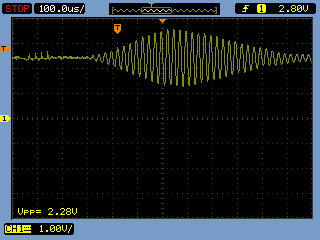
\includegraphics[width = 0.4\textwidth]{billeder/PGA}
\caption{Burst set mellem PGA og mixer}
\label{fig:PGA}
\end{figure}
\begin{figure}[hbpt]
\centering
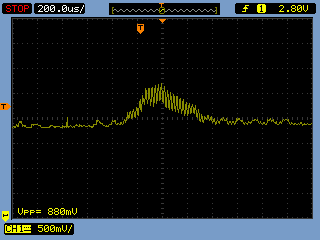
\includegraphics[width = 0.4\textwidth]{billeder/mixer}
\caption{Burst set mellem mixer og delta-sigma}
\label{fig:mixer}
\end{figure}
\begin{figure}[hbpt]
\centering
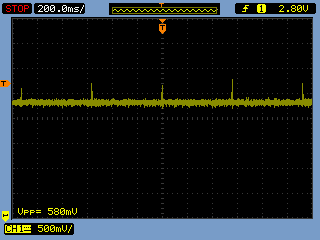
\includegraphics[width = 0.4\textwidth]{billeder/mixer2}
\caption{gentagene burst set mellem mixer og delta-sigma}
\label{fig:mixer2}
\end{figure}
\begin{figure}[hbpt]
\centering
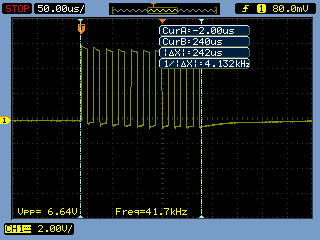
\includegraphics[width = 0.4\textwidth]{billeder/burst}
\caption{Burst sendt fra PSoC'en}
\label{fig:flereburstpsoc}
\end{figure}
\begin{figure}[hbpt]
\centering
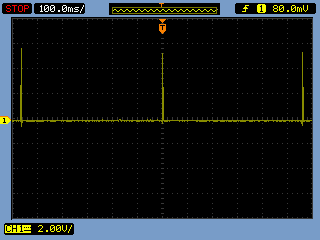
\includegraphics[width = 0.4\textwidth]{billeder/gentageneburst}
\caption{gentagene burst sendt fra PSoC'en}
\label{fig:burstpsoc}
\end{figure}
\begin{figure}[hbpt]
\centering
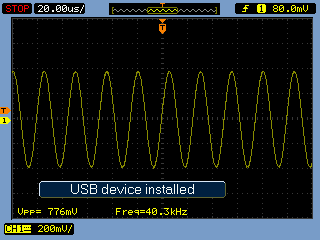
\includegraphics[width = 0.4\textwidth]{billeder/transmittertest}
\caption{40kHz signal fra transmitter set på receiver}
\label{fig:transmittertest}
\end{figure}

\section{Test kode til VBTE}

\lstset{language=C++,                % choose the language of the code
  numbers=left,                   % where to put the line-numbers
  stepnumber=1,                   % the step between two line-numbers.        
  numbersep=10pt,                  % how far the line-numbers are from the code
  backgroundcolor=\color{white},  % choose the background color. You must add \usepackage{color}
  showspaces=false,               % show spaces adding particular underscores
  showstringspaces=false,         % underline spaces within strings
  showtabs=false,                 % show tabs within strings adding particular underscores
  tabsize=2,                      % sets default tabsize to 2 spaces
  captionpos=b,                   % sets the caption-position to bottom
  breaklines=true,                % sets automatic line breaking
  breakatwhitespace=true,         % sets if automatic breaks should only happen at whitespace
  title=\lstname,                 % show the filename of files included with \lstinputlisting;
}
\texttt{\lstinputlisting{Test/test_VBTE.c}}





